\documentclass[11pt]{article}
\usepackage[utf8]{inputenc}
\usepackage[T1]{fontenc}
\usepackage[francais]{babel}
\usepackage[francais]{layout}
\usepackage{hyperref}
\selectlanguage{french}

% NE PAS CHANGER !!
\ifx \public \undefined \def\public{etudiants} \fi
\usepackage[\public]{tps}
\usepackage{tikz}
\projettrue

% Numéro du TP
\newcommand{\numtd}{Project I: Computer Architecture }
% Titre du TP
\newcommand{\titretd}{Construction of a real computer}
\def\tup#1{\langle #1\rangle}
\begin{document}

\entete{\numtd}{\titretd}

\section{Project Guidelines}
For the project, you need to send the completed files in the zipped folder available at \url{https://www.amritasuresh.github.io/teaching/comparch.tar.gz}. The assignments for Sections \ref{sec:gates} and \ref{sec:computer} require the \texttt{.hdl} files to be sent, along with the \texttt{.asm} file for Section 3. The deadline for the submission is \textbf{14h00 CET 29th November 2021}. Each question is marked with points. Don't worry about them too much, it is more a guideline for the effort required per question, as opposed to the grade. 

\section{Recap: Introduction to Logic Gates}
\label{sec:gates}

\subsection{Introduction}
Using the chips from the TPs 2 and 3, we will now build some other components in a similar fashion. The \texttt{.hdl} along with the test cases are available in the \texttt{Project Logic Gates} folder of the zipped file. For highest points, try to implement the chips using the number of instructions specified. If you cannot find the optimal implementation, you will still be awarded partial points for a correct implementation. Note: All files related to this exercise are available on \texttt{comparch/assignment/project/logicgates}.

\subsection{Task}
For this section, program the chips in the following order (assuming you have the chips from the TPs).

\begin{enumerate}
	\item \texttt{Xnor} (2 instructions) \hspace*{\fill} \texttt{\small  1 point}
	\item \texttt{Or16Way} (3 instructions) \hspace*{\fill} \texttt{\small  1 point}
	\item \texttt{CarryLookahead4} \hspace*{\fill} \texttt{\small  4 points}
	
	This is a 4-bit adder with the lookahead logic that you have seen in class. To learn more, refer to the circuit description available in the folder \texttt{logicgates}. 
	\emph{Note:} Any implementation will be awarded full points. Feel free to add other chips if it simplifies things for you.
	\item \texttt{UnaryALU} (4 instructions)  \hspace*{\fill} \texttt{\small  2 points}
	\item \texttt{ALU} (8 instructions) \hspace*{\fill} \texttt{\small  4 points}
	
	With some chips constructed earlier in this task, we can build a more compact ALU.
	\item \texttt{Subtractor} (1 instruction) \hspace*{\fill} \texttt{\small  2 points}
\end{enumerate}

\section{Machine Language Programming}

\subsection{Overview}
In computer programming, machine code is any low-level programming language, consisting of machine language instructions, which is used to control a computer's central processing unit (CPU). Each instruction causes the CPU to perform a very specific task, such as a load, a store, a jump, or an arithmetic logic unit (ALU) operation on one or more units of data in the CPU's registers or memory.
Each hardware platform is designed to execute a certain machine language, expressed using agreed upon binary codes. Writing programs directly in binary code is a possible, but it is extremely tedious.
 Instead, we can write such programs in a low-level symbolic language, called assembly,
and have them translated into binary code by a program called an assembler. In this project, you
will write some low-level assembly programs, and will be forever thankful for high-level languages
like C and Python. (Actually, assembly programming can be a lot of fun, if you are in the right
mood; it’s an excellent brain teaser, and it allows you to control the underlying machine directly
and completely.)

\subsection{Introduction}

To get a taste of low-level programming in machine language, and to get acquainted with the
 computer platform which we have been constructing for the past two TPs. In the process of working on this project, you will become familiar with
the assembly process — translating from symbolic language to machine-language — and you will
appreciate visually how native binary code executes on the target hardware platform. Moreover, you will get acquainted with how the instructions are written and interpreted by the machine. These lessons
will be learned in the context of writing and analyzing the low-level programs described below.

\subsection{Resources}
Note: All files related to this exercise are available on \texttt{comparch/assignment/project/machinelanguage}.
The assembly language is described in detail in the instruction manual in the \texttt{Machine Language} folder of the Project. I suggest taking a look at this tutorial before you start this section of the project.

To run your program, you will need two tools: the supplied Assembler — a program that translates programs written in the assembly language
into binary code, and the supplied CPU Emulator — a program that runs binary code on a simulated platform. These are included in the zipped file. To use the GUI of the CPU Emulator, run \texttt{tools/CPUEmulator.sh}. You can have a look at the CPU Emulator Tutorial in case you want to get an idea of how it works. If not, you can just learn by running the tool and experimenting.

\subsection{Task}
\subsubsection{Warmup}
We now move to the \texttt{Machine Language} folder of our Project. To first get a little acquainted with the machine language, let us look at some more examples. What do the following programs in machine language compute?
\begin{enumerate}
	\item \begin{verbatim*}
		@2
		D=A 
		@3
		D=D+A 
		@0
		M=D 
	\end{verbatim*} \hspace*{\fill} \texttt{\small  2 points}
\item \begin{verbatim}
	@R0
	D=M              // D = first number
	@R1
	D=D-M            // D = first number - second number
	@OUTPUT_FIRST
	D;JGT            // if D>0 goto output_first
	@R1
	D=M              // D = second number
	@OUTPUT_D
	0;JMP            // goto output_d
	(OUTPUT_FIRST)
	@R0             
	D=M              // D = first number
	(OUTPUT_D)
	@R2
	M=D              // M[2] = D 
	(INFINITE_LOOP)
	@INFINITE_LOOP
	0;JMP            // infinite loop
	
\end{verbatim} \hspace*{\fill} \texttt{\small  3 points}
\end{enumerate}

\subsubsection{Multiplying 2 Numbers}
Write and test the following program described below. When executed on the CPU Emulator, your
program should generate the results mandated by the specified tests. \hspace*{\fill} \texttt{\small  5 points}

\subsection*{Description:}  

\texttt{mult.asm} : In the computer that we build, the top 16 RAM words (RAM[0]...RAM[15]) are also referred to as R0...R15. 

With this terminology in mind, this program computes the value R0*R1 and stores the result in R2.

The program assumes that R0$>=0$, R1>$=0$, and R0*R1$<32768$. Your program need not test these conditions, but rather assume that they hold.

\subsection*{Guidelines}
\begin{itemize}
	\item Use a plain text editor to write your \texttt{mult.asm}  program using the assembly language specified in Appendix A.
	\item Use the supplied Assembler to translate your \texttt{mult.asm} program, producing a file containing binary instructions.
	\item Next, load the supplied \texttt{mult.tst} script into the CPU Emulator. This script loads the Mult program, and executes it.
	\item Run the script. If you get any errors, debug and edit your \texttt{mult.asm} program. Then assemble the program, re-run the \texttt{mult.tst} script, etc.
\end{itemize}


\section{Computer}
\label{sec:computer}
\subsection{Introduction}
In previous projects we’ve built the computer’s basic processing and storage devices (ALU and
RAM, respectively). In this project we will put everything together, yielding the complete 
Hardware Platform. The result will be a general-purpose computer that can run any program that
you fancy.

\subsection{Task}

Note: All files related to this exercise are available on \texttt{comparch/assignment/project/computer}.

We will reuse the RAM built in the previous TP as well as our ALU to build a \textit{real} computer. Our computer will use two external peripherals: a keyboard and a screen (which are built-in), and whose specification is given to you respectively in Fig.~\ref{fig:keyboard} and Fig.~\ref{fig:screen}. Note that the Hardware Simulator manages the inputs /outputs for you. In our case, we will not take care of the entries. In the Hardware Simulator, under the option \textbf{View} you can select \textbf{Screen} to see what some tests produce (like \texttt{ComputerRect-external.tst}). Implement the chips in the following order:

\begin{enumerate}
\item \texttt{Memory} (7 instructions) \hspace*{\fill} \texttt{\small  5 points}
\item \texttt{CPU} (20 instructions) \hspace*{\fill} \texttt{\small  10 points}
\item \texttt{Computer} (3 instructions)  \hspace*{\fill} \texttt{\small  3 points}
\end{enumerate}

In order to help you, you will find in Fig.~\ref{fig:cpu}, a diagram which summarizes the internal behavior of the CPU, and also the computer.

\begin{figure}[h!]
	\centering
	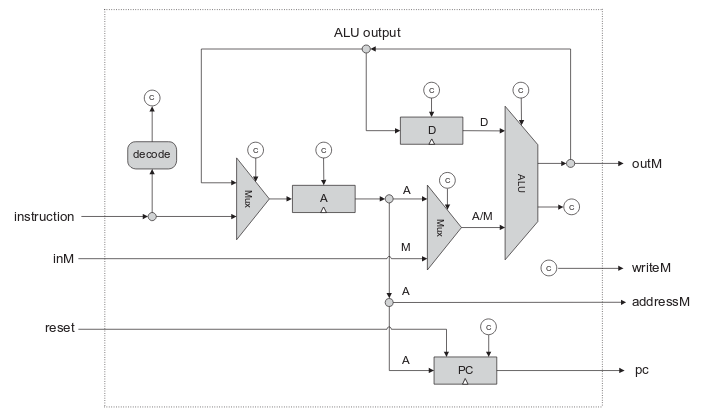
\includegraphics[scale=0.5]{pictures/cpu.png}
	\caption{CPU}
	\label{fig:cpu}
\end{figure}

\begin{figure}[h!]
	\centering
	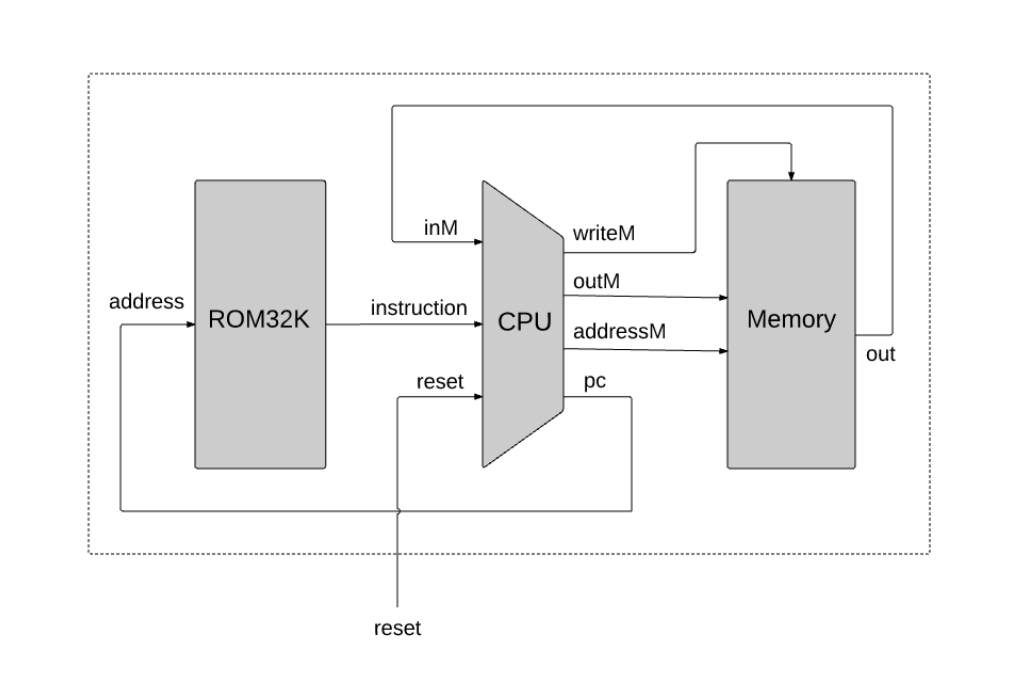
\includegraphics[scale=0.5]{pictures/cmp.png}
	\caption{Computer}
	\label{fig:comp}
\end{figure}


\begin{figure}[]
  \centering
\begin{verbatim}
Chip Name:
Keyboard    // Memory map of the physical keyboard.
            // Outputs the code of the currently
            // pressed key.
Output:
out[16]     // The ASCII code of the pressed key, or
            // one of the special codes
Function:
Outputs the code of the key presently pressed on the
physical keyboard.
Comment:
This chip is continuously being refreshed from a
physical keyboard unit (simulators must simulate this
service).
\end{verbatim}

  \caption{Keyboard}
  \label{fig:keyboard}
\end{figure}
\begin{figure}[]
  \centering
\begin{verbatim}
Chip Name:
Screen       // Memory map of the physical screen
Inputs:
in[16],      // What to write
load,        // Write-enable bit
address[13]  // Where to write
Output:
out[16]      // Screen value at the given address
Function:
Functions exactly like a 16-bit 8K RAM:
1. out(t)=Screen[address(t)](t)
2. If load(t-1) then Screen[address(t-1)](t)=in(t-1)
(t is the current time unit, or cycle)
Comment:
Has the side effect of continuously refreshing a 256
by 512 black-and-white screen (simulators must
simulate this device). Each row in the physical
screen is represented by 32 consecutive 16-bit words,
starting at the top left corner of the screen. Thus
the pixel at row r from the top and column c from the
left (0<=r<=255, 0<=c<=511) reflects the c%16 bit
(counting from LSB to MSB) of the word found at
Screen[r*32+c/16].
\end{verbatim}

  \caption{Screen}
  \label{fig:screen}
\end{figure}

 In addition, in our architecture, we must load our program in memory which will be different from the \texttt{RAM}. Here it will be the \texttt{ROM}. For that, we will also use a \textit{built-in} chip which will simulate this component see Fig.~\ref{fig:rom}.
 \begin{figure}[]
 	\centering
 	\begin{verbatim}
 		Chip Name:
 		ROM32K            // 16-bit read-only 32K memory
 		Input:
 		address[15]       // Address in the ROM
 		Output:
 		out[16]           // Value of ROM[address]
 		Function:
 		out=ROM[address]  // 16-bit assignment
 		Comment:
 		The ROM is preloaded with a machine language program.
 		Hardware implementations can treat the ROM as a
 		built-in chip. Software simulators must supply a
 		mechanism for loading a program into the ROM.
 	\end{verbatim}
 	\caption{ROM}
 	\label{fig:rom}
 \end{figure}
\pagebreak

We now look more closely at the specifications of the machine language. Our objective is to come up with a logic gate architecture capable of (i) executing a given instruction, and (ii) determining which
instruction should be fetched and executed next. In order to do so, the proposed CPU
implementation includes an ALU chip capable of computing arithmetic/logical functions, a set of
registers, a program counter, and some additional gates designed to help decode, execute, and
fetch instructions. Since all these building blocks were already built in previous chapters, the
key question that we face now is how to arrange and connect them in a way that effects the
desired CPU operation. 

The architecture shown in Fig.~\ref{fig:cpu} is used to perform three classical CPU tasks: decoding
the current instruction, executing the current instruction, and deciding which instruction to fetch
and execute next. We now turn to describe these three tasks.

\subsection*{Instruction decoding}
The 16-bit value of the CPU’s instruction input represents either an \texttt{A-instruction} or a \texttt{C-instruction}. In order to figure out the semantics of this instruction, we can parse, or unpack it,
into the following fields: \texttt{ixxaccccccdddjjj}. The \texttt{i}-bit (also known as opcode) codes the
instruction type, which is either 0 for an \texttt{A-instruction} or 1 for a \texttt{C-instruction}. In case of an \texttt{A-instruction}, the entire instruction represent the 16-bit value of the constant that should be loaded
into the A register. In case of a \texttt{C-instruction}, the \texttt{a}- and \texttt{c}-bits code the comp part of the instruction, while the \texttt{d}- and \texttt{j}-bits code the \texttt{dest} and \texttt{jump} parts of the instruction, respectively
(the \texttt{x}-bits are not used, and can be ignored). 

\subsection*{Instruction execution}
The decoded fields of the instruction (\texttt{i}-, \texttt{a}-, \texttt{c}-, \texttt{d}-, and \texttt{j}-bits) are routed simultaneously to various parts of the CPU architecture, where they cause different chip-parts to do what they are supposed to do in order to execute either the A- or the C-instruction, as mandated by the
machine language specification. In the case of a C-instruction, the single \texttt{a}-bit determines
whether the ALU will operate on the A register input or on the M input, and the six \texttt{c}-bits
determine which function the ALU will compute. The three \texttt{d}-bits are used to determine which
registers should “accept” the ALU resulting output, and the three \texttt{j}-bits are used to for branching
control, which can be seen in the following figures.

\begin{figure}[h!]
	\centering
	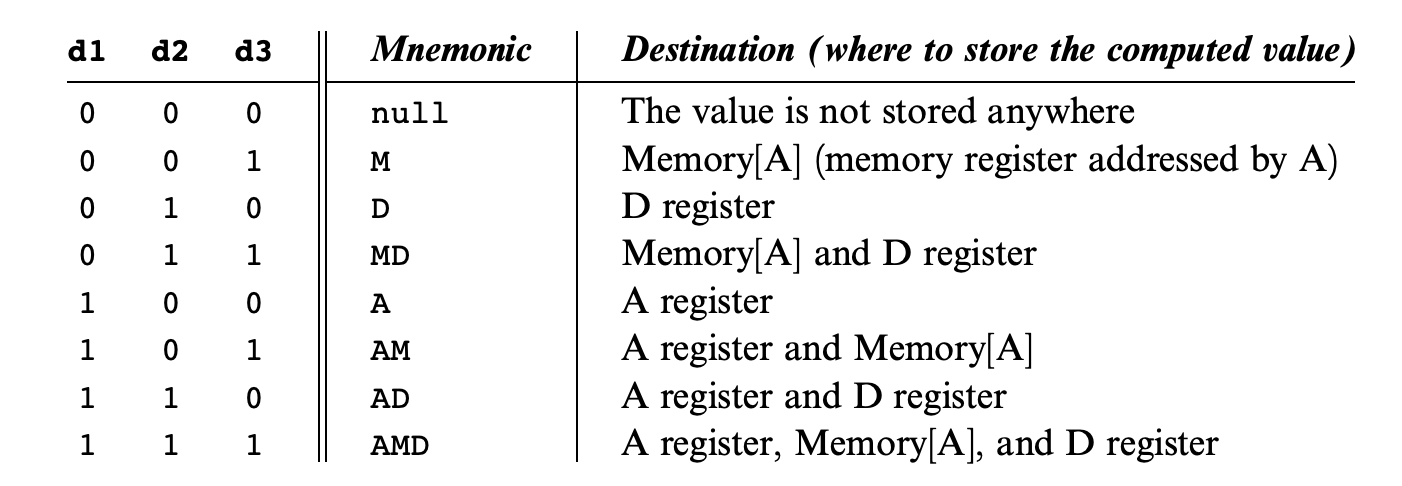
\includegraphics[scale=0.5]{pictures/dst.png}
	\caption{The dest field of the C-instruction}
	\label{fig:dst}
\end{figure}

\begin{figure}[h!]
	\centering
	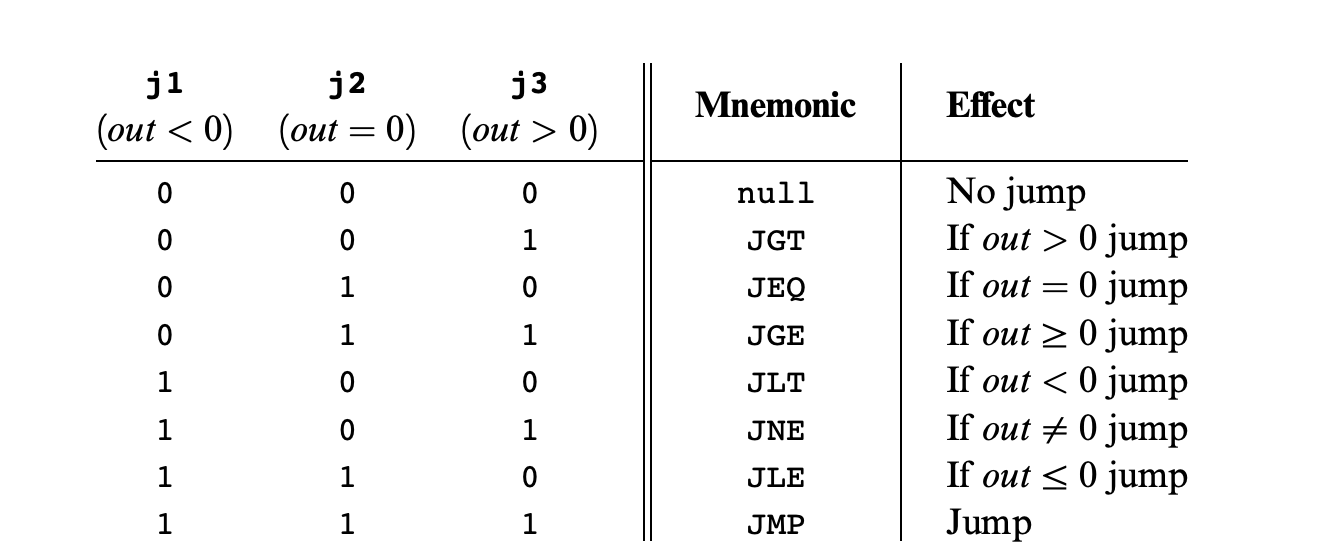
\includegraphics[scale=0.5]{pictures/jmp.png}
	\caption{The jump field of the C-instruction. Out refers to the ALU output (resulting from
		the instruction’s comp part), and jump implies ‘‘continue execution with the instruction
		addressed by the A register.’’}
	\label{fig:jmp}
\end{figure}




\end{document}
